\documentclass{article}
\usepackage{tikz}
\usepackage{pgfplots}
\usepackage{svg}
\usepackage{amsmath}
\usepackage{array}
\usepackage[skins]{tcolorbox}
\usepackage[version=4]{mhchem}
\usepackage[a4paper, total={6in, 9in}]{geometry}
\usepackage{fourier}
\usepackage{xymtex}
\usepackage{textcomp}
\usepackage{eurosym}
\usepackage{caption}
\usepackage{longtable}
\usepackage{float}
\usepackage{attachfile}
\usepackage{multirow}
\usepackage{amsfonts} 
\usepackage{tabularray}
\usepackage{colortbl}
\usepackage{xcolor}
\usepackage{graphicx}
\usepackage[table]{xcolor}
\UseTblrLibrary{booktabs}
\usepackage[bottom]{footmisc}
\pgfplotsset{compat=1.18}
\usepackage{siunitx}
\usepgfplotslibrary{colormaps}


% Indice
\renewcommand*\contentsname{Indice}
\setcounter{tocdepth}{3}
%\setcounter{secnumdepth}{2}

%Regole tabelle
\captionsetup[table]{name=Tabella}
\usepackage{booktabs}
\usepackage{caption}
\usepackage{float}
\usepackage{titlesec}
\usepackage{capt-of}



%colori custom
\definecolor{myyellow}{RGB}{245, 215, 66} 
\definecolor{myred}{RGB}{255, 115, 69} 
\definecolor{mylightblue}{RGB}{134, 213, 247} 
\definecolor{myblue}{RGB}{56, 103, 214} 



%sfondi colorati
\newcommand{\giallo}[1]{\colorbox{myyellow}{$\displaystyle #1$}}
\newcommand{\rosso}[1]{\colorbox{myred}{$\displaystyle #1$}}
\newcommand{\azzurro}[1]{\colorbox{mylightblue}{$\displaystyle #1$}}
\newcommand{\blu}[1]{\colorbox{myblue}{$\displaystyle #1$}}

\title{Relazione di laboratorio - Periodo di un pendolo semplice}
\author{Federico Cesari}
\date{Aprile 2024}




%%%%%%%%%%%%%%%%%%%%%%%%%%%%%%%%%%%%%%%%%%%%%%%%%%%%%%%%%
%%				INIZIO DOC
%%%%%%%%%%%%%%%%%%%%%%%%%%%%%%%%%%%%%%%%%%%%%%%%%%%%%%%%%


\begin{document}
	\begin{titlepage}
   \begin{center}
       \vspace*{1cm}
        
       \textbf{\LARGE Relazione di laboratorio - Esperienza di Poisson}
       
       \vspace{0.3cm}
       \large \textit{Rate di una sorgente radioattiva} \\
       
       \vspace{0.5cm}
       \Large Federico Cesari \\
       
       \small 1096759

			
		\vspace{1cm}
		\begin{center}
			\includegraphics[scale=1.2]{geiger.jpeg}	
		\end{center}
		
		

       \vfill
            
       
            
       \vspace{0.8cm}
     
       
            
       corso A\\
       Università degli studi di Torino, Torino\\
       3 marzo 2024\\
       
            
   \end{center}
\end{titlepage}

	\tableofcontents
	
	%\newpage
	%\textcolor{white}{.}
	%\vfill
	\newpage
	\section*{Scopo dell’esperienza e aspettative teoriche}
	\section*{Strumentazione}
	
	\newpage
	\section{Prima presa dati}
		\subsection{Cilindro metallico}

		\begin{center}
			\textit{tabella T1 } \textit{ tabella crescita } \textit{ tabella Teq}
		\end{center}
		\begin{center}
				\begin{figure}[H]
					\centering
					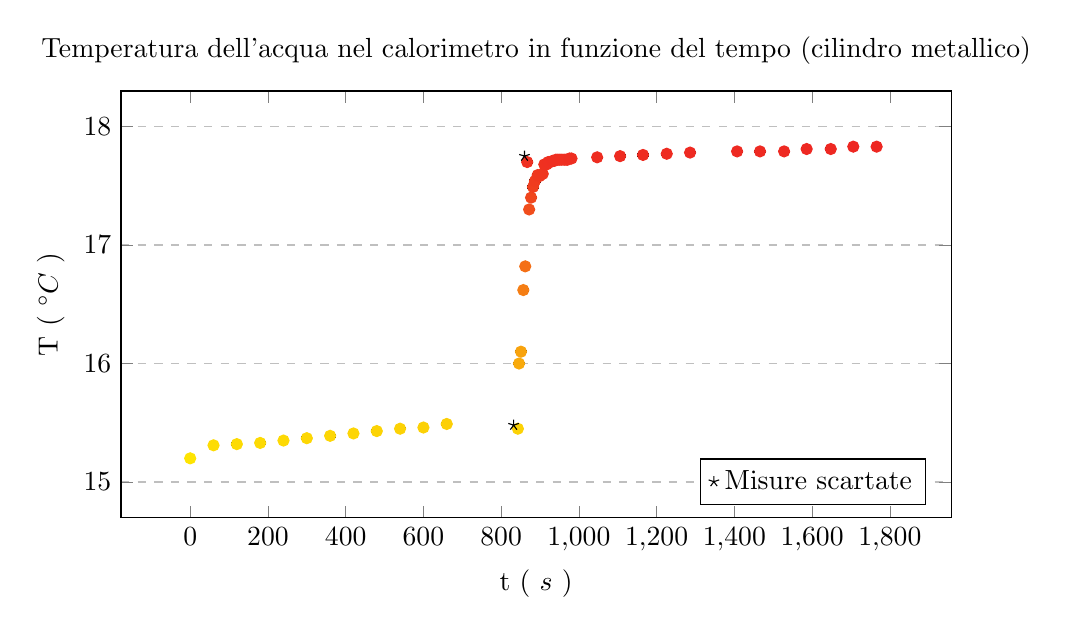
\begin{tikzpicture}
						\begin{axis}[
							title={Temperatura dell'acqua nel calorimetro in funzione del tempo (cilindro metallico)},
							xlabel={t ( $s$ )},
							ylabel={T ( $^\circ C$ )},
							xmin=0, xmax=1780,
							ymin=15, ymax=18,
							xtick={},
							ytick={},
							legend pos=south east,
							ymajorgrids=true,
							grid style=dashed,
							enlargelimits=0.1,
							width=\textwidth,
							height=7cm,
							point meta min=15,
							point meta max=18,
							colormap={yellowred}{
								color(0cm)=(yellow)
								color(1cm)=(red)
							},
							]
							
							% Define the data
							\pgfplotstableread{
								x y yerr
								0 15.2 0.01
								60 15.31 0.01
								120 15.32 0.01
								180 15.33 0.01
								240 15.35 0.01
								300 15.37 0.01
								360 15.39 0.01
								420 15.41 0.01
								480 15.43 0.01
								540 15.45 0.01
								600 15.46 0.01
								660 15.49 0.01
								843 15.45 0.01
								846 16.0 0.01
								851 16.1 0.01
								857 16.62 0.01
								862 16.82 0.01
								867 17.7 0.01
								872 17.3 0.01
								877 17.4 0.01
								882 17.49 0.01
								887 17.54 0.01
								894 17.59 0.01
								898 17.58 0.01
								901 17.59 0.01
								907 17.6 0.01
								911 17.68 0.01
								917 17.68 0.01
								921 17.7 0.01
								927 17.7 0.01
								932 17.71 0.01
								937 17.71 0.01
								941 17.72 0.01
								946 17.72 0.01
								951 17.72 0.01
								956 17.72 0.01
								962 17.72 0.01
								967 17.72 0.01
								971 17.72 0.01
								976 17.73 0.01
								981 17.73 0.01
								1047 17.74 0.01
								1106 17.75 0.01
								1165 17.76 0.01
								1226 17.77 0.01
								1286 17.78 0.01
								1407 17.79 0.01
								1466 17.79 0.01
								1528 17.79 0.01
								1586 17.81 0.01
								1648 17.81 0.01
								1706 17.83 0.01
								1766 17.83 0.01
							} \datatable
							
							% Plot the data with gradient
							\addplot[
							scatter, 
							only marks, 
							scatter src=explicit,
							scatter/use mapped color={
								draw=mapped color,
								fill=mapped color
							},
							error bars/.cd,
							y dir=both, y explicit
							]
							table[x=x, y=y, y error=yerr, meta=y] {\datatable};
							\addplot[
							only marks,
							mark=star,
							]
							coordinates {(832, 15.48)};
							\addplot[
							only marks,
							mark=star,
							]
							coordinates {(860, 17.75)};
							\legend{,,Misure scartate}
						\end{axis}
					\end{tikzpicture}
				\end{figure}
		\end{center}
		
		\begin{center}
			\begin{figure}[H]
				\centering
				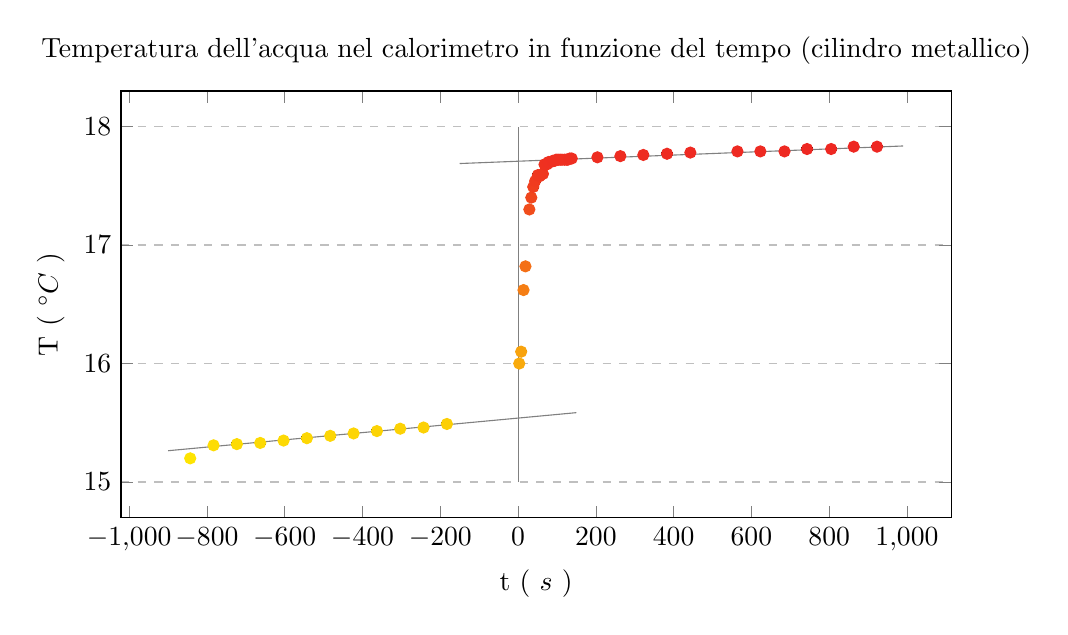
\begin{tikzpicture}
					\begin{axis}[
						title={Temperatura dell'acqua nel calorimetro in funzione del tempo (cilindro metallico)},
						xlabel={t ( $s$ )},
						ylabel={T ( $^\circ C$ )},
						xmin=-843, xmax=936,
						ymin=15, ymax=18,
						xtick={},
						ytick={},
						legend pos=south east,
						ymajorgrids=true,
						grid style=dashed,
						enlargelimits=0.1,
						width=\textwidth,
						height=7cm,
						point meta min=15,
						point meta max=18,
						colormap={yellowred}{
							color(0cm)=(yellow)
							color(1cm)=(red)
						},
						]
						
						% Define the data
						\pgfplotstableread{
							x y yerr
							-843 15.2 0.01
							-783 15.31 0.01
							-723 15.32 0.01
							-663 15.33 0.01
							-603 15.35 0.01
							-543 15.37 0.01
							-483 15.39 0.01
							-423 15.41 0.01
							-363 15.43 0.01
							-303 15.45 0.01
							-243 15.46 0.01
							-183 15.49 0.01
							3 16.0 0.01
							8 16.1 0.01
							14 16.62 0.01
							19 16.82 0.01
							29 17.3 0.01
							34 17.4 0.01
							39 17.49 0.01
							44 17.54 0.01
							51 17.59 0.01
							55 17.58 0.01
							58 17.59 0.01
							64 17.6 0.01
							68 17.68 0.01
							74 17.68 0.01
							78 17.7 0.01
							84 17.7 0.01
							89 17.71 0.01
							94 17.71 0.01
							98 17.72 0.01
							103 17.72 0.01
							108 17.72 0.01
							113 17.72 0.01
							119 17.72 0.01
							124 17.72 0.01
							128 17.72 0.01
							133 17.73 0.01
							138 17.73 0.01
							204 17.74 0.01
							263 17.75 0.01
							322 17.76 0.01
							383 17.77 0.01
							443 17.78 0.01
							564 17.79 0.01
							623 17.79 0.01
							685 17.79 0.01
							743 17.81 0.01
							805 17.81 0.01
							863 17.83 0.01
							923 17.83 0.01
						} \datatable
						
						% Plot the data with gradient
						\addplot[
						scatter, 
						only marks, 
						scatter src=explicit,
						scatter/use mapped color={
							draw=mapped color,
							fill=mapped color
						},
						error bars/.cd,
						y dir=both, y explicit
						]
						table[x=x, y=y, y error=yerr, meta=y] {\datatable};
						% Add vertical line at x=0
						\addplot [
						domain=15:18,
						samples=2,
						color=gray,
						]
						coordinates {(0,15) (0,18)};
						
						% Add line y = 15.539645 + 0.000306x
						\addplot [
						domain=-900:150,
						samples=100,
						color=gray,
						]
						{15.539645 + 0.000306*x};
						
						% Add line y = 17.707 + 0.00013x
						\addplot [
						domain=-150:990,
						samples=100,
						color=gray,
						]
						{17.707 + 0.00013*x};
					\end{axis}
				\end{tikzpicture}
			\end{figure}
		\end{center}
		\[ 
		\giallo{\boldsymbol{T_{1} = 15.54 \pm 0.01} }\footnotemark
		\]
		\[ 
		\rosso{\boldsymbol{T_{\text{eq}} = 17.71	\pm 0.02}}
		\]
		\footnote{Valore misurato \(T_{1} = 15.539645	\pm 0.00451\)}
		
		
		\subsection{Massa d'acqua}
		
		\begin{center}
				\begin{figure}[H]
					\centering
					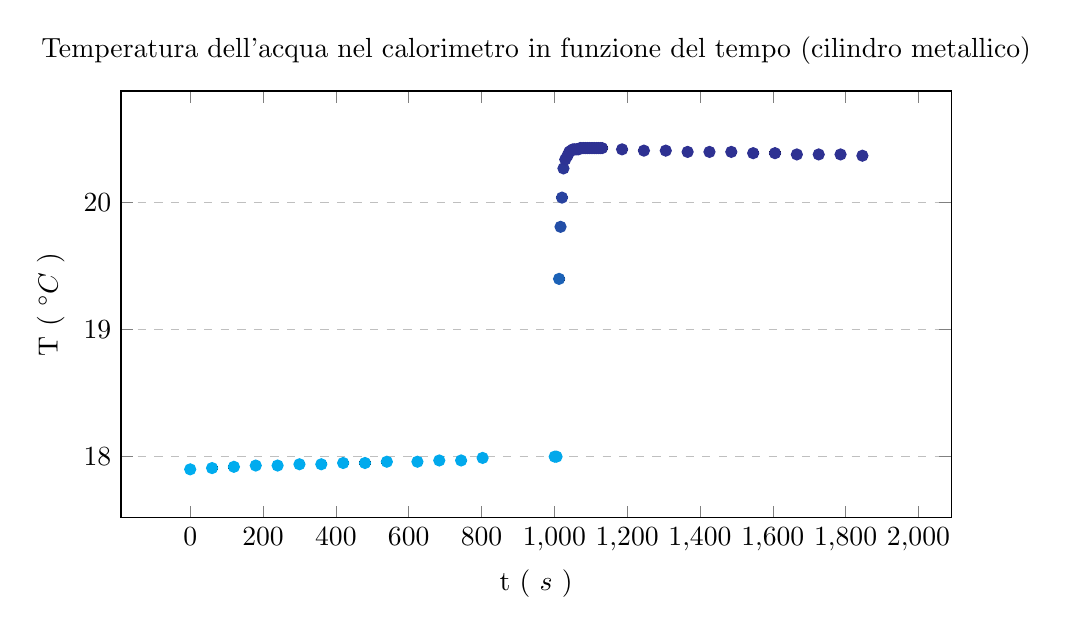
\begin{tikzpicture}
						\begin{axis}[
							title={Temperatura dell'acqua nel calorimetro in funzione del tempo (cilindro metallico)},
							xlabel={t ( $s$ )},
							ylabel={T ( $^\circ C$ )},
							xmin=0, xmax=1900,
							ymin=17.8, ymax=20.6,
							xtick={},
							ytick={},
							legend pos=north west,
							ymajorgrids=true,
							grid style=dashed,
							enlargelimits=0.1,
							width=\textwidth,
							height=7cm,
							point meta min=17.9,
							point meta max=20.4,
							colormap={yellowred}{
								color(0cm)=(cyan)
								color(1cm)=(blue)
							},
							]
							
							% Define the data
							\pgfplotstableread{
								x y yerr
								0.00 17.90 0.01
								60.00 17.91 0.01
								120.00 17.92 0.01
								180.00 17.93 0.01
								240.00 17.93 0.01
								300.00 17.94 0.01
								360.00 17.94 0.01
								420.00 17.95 0.01
								480.00 17.95 0.01
								540.00 17.96 0.01
								624.00 17.96 0.01
								684.00 17.97 0.01
								744.00 17.97 0.01
								803.00 17.99 0.01
								1001.00 18.00 0.01
								1006.00 18.00 0.01
								1013.00 19.4 0.01
								1017.00 19.81 0.01
								1021.00 20.04 0.01
								1025.00 20.27 0.01
								1030.00 20.34 0.01
								1036.00 20.37 0.01
								1041.00 20.40 0.01
								1046.00 20.41 0.01
								1051.00 20.42 0.01
								1056.00 20.42 0.01
								1061.00 20.42 0.01
								1066.00 20.42 0.01
								1071.00 20.43 0.01
								1076.00 20.43 0.01
								1081.00 20.43 0.01
								1086.00 20.43 0.01
								1091.00 20.43 0.01
								1096.00 20.43 0.01
								1101.00 20.43 0.01
								1106.00 20.43 0.01
								1111.00 20.43 0.01
								1116.00 20.43 0.01
								1121.00 20.43 0.01
								1126.00 20.43 0.01
								1131.00 20.43 0.01
								1186.00 20.42 0.01
								1246.00 20.41 0.01
								1306.00 20.41 0.01
								1366.00 20.40 0.01
								1426.00 20.40 0.01
								1486.00 20.40 0.01
								1546.00 20.39 0.01
								1606.00 20.39 0.01
								1666.00 20.38 0.01
								1726.00 20.38 0.01
								1786.00 20.38 0.01
								1846.00 20.37 0.01
								
							} \datatable
							
							% Plot the data with gradient
							\addplot[
							scatter, 
							only marks, 
							scatter src=explicit,
							scatter/use mapped color={
								draw=mapped color,
								fill=mapped color
							},
							error bars/.cd,
							y dir=both, y explicit
							]
							table[x=x, y=y, y error=yerr, meta=y] {\datatable};
						\end{axis}
					\end{tikzpicture}
				\end{figure}
		\end{center}
		
		\begin{center}
			\begin{figure}[H]
				\centering
				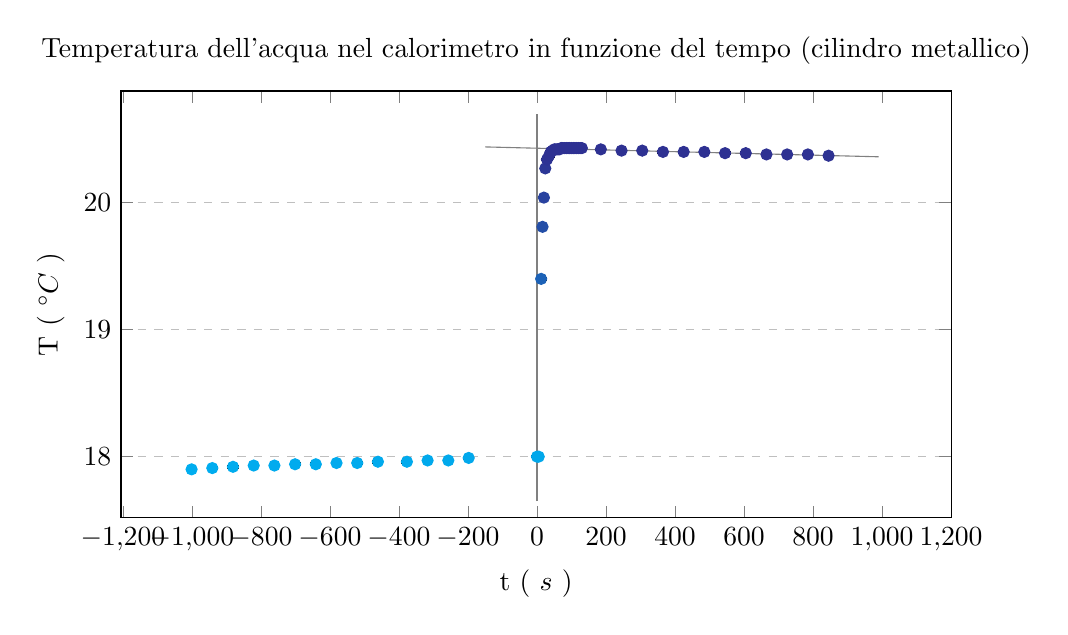
\begin{tikzpicture}
					\begin{axis}[
						title={Temperatura dell'acqua nel calorimetro in funzione del tempo (cilindro metallico)},
						xlabel={t ( $s$ )},
						ylabel={T ( $^\circ C$ )},
						xmin=-1005, xmax=1000,
						ymin=17.8, ymax=20.6,
						xtick={},
						ytick={},
						legend pos=north west,
						ymajorgrids=true,
						grid style=dashed,
						enlargelimits=0.1,
						width=\textwidth,
						height=7cm,
						point meta min=17.9,
						point meta max=20.4,
						colormap={yellowred}{
							color(0cm)=(cyan)
							color(1cm)=(blue)
						},
						]
						
						% Define the data
						\pgfplotstableread{
							x y yerr
							-1001 17.90 0.01
							-941 17.91 0.01
							-881 17.92 0.01
							-821 17.93 0.01
							-761 17.93 0.01
							-701 17.94 0.01
							-641 17.94 0.01
							-581 17.95 0.01
							-521 17.95 0.01
							-461 17.96 0.01
							-377 17.96 0.01
							-317 17.97 0.01
							-257 17.97 0.01
							-198 17.99 0.01
							0 18.00 0.01
							5 18.00 0.01
							12 19.4 0.01
							16 19.81 0.01
							20 20.04 0.01
							24 20.27 0.01
							29 20.34 0.01
							35 20.37 0.01
							40 20.40 0.01
							45 20.41 0.01
							50 20.42 0.01
							55 20.42 0.01
							60 20.42 0.01
							65 20.42 0.01
							70 20.43 0.01
							75 20.43 0.01
							80 20.43 0.01
							85 20.43 0.01
							90 20.43 0.01
							95 20.43 0.01
							100 20.43 0.01
							105 20.43 0.01
							110 20.43 0.01
							115 20.43 0.01
							120 20.43 0.01
							125 20.43 0.01
							130 20.43 0.01
							185 20.42 0.01
							245 20.41 0.01
							305 20.41 0.01
							365 20.40 0.01
							425 20.40 0.01
							485 20.40 0.01
							545 20.39 0.01
							605 20.39 0.01
							665 20.38 0.01
							725 20.38 0.01
							785 20.38 0.01
							845 20.37 0.01
							
						} \datatable
						
						% Plot the data with gradient
						\addplot[
						scatter, 
						only marks, 
						scatter src=explicit,
						scatter/use mapped color={
							draw=mapped color,
							fill=mapped color
						},
						error bars/.cd,
						y dir=both, y explicit
						]
						table[x=x, y=y, y error=yerr, meta=y] {\datatable};
						
						% Add vertical line at x=0
						\addplot [
						domain=15:18,
						samples=2,
						color=gray,
						]
						coordinates {(0,17.65) (0,20.7)};
					
						\addplot [
						domain=-150:990,
						samples=100,
						color=gray,
						]
						{20.429 - 0.000068181818181745*x};
					\end{axis}
				\end{tikzpicture}
			\end{figure}
		\end{center}
		\begin{minipage}{\textwidth}
		\[ 
		\azzurro{\boldsymbol{T_{1} = 18.00 \pm	0.01} }
		\]
		\end{minipage}
		\begin{minipage}{\textwidth}
			\[ 
			\blu{\boldsymbol{T_{\text{eq}} = 20.43 \pm 0.01} }\footnotemark
			\]
		\end{minipage}
		
		\footnotetext{Valore rilevato \(T_{\text{eq}} = 20.429 \pm 0.002\). l'errore è minore della sensibilità del termometro quindi riporto la temperatura con due cifre decimali e come errore la sensibilità.}
		
		
			
	\subsection{Analisi errori}
	
	\newpage
	\section{Seconda presa dati}
	
	\newpage
	\section{Confronto masse equivalenti e calori specifici}
	
	\newpage
	\section{Errori sistematici}
	\subsection{Influenza agitatore}
	\subsection{Calore disperso}
	
	\newpage
	\section{Appendice}
	\subsection{Calcolo \(T_{1}\) e \(T_{\text{eq}}\) con covarianze}
	Al fine di semplificare la ricerca di temperatura iniziale e temperatura di equilibrio è utile traslare i grafici portando l'istante d'immersione (prima del corpo poi della massa d'acqua) sullo \(0\). In questo modo le due temperature risultano essere semplicemente i termini noti delle rette di best-fit. \\
	
	Senza ricorrere alla traslazione è possibile ricavare i due valori trovando l'intersezione delle due rette di best-fit con la retta \(x=t_{\text{i}}\) istante di immersione. In questo caso però il punto dove le rette intersecano \(x=t_{\text{i}}\) dipenderà dai parametri delle due rette  \(\boldsymbol{a}\) e \(\boldsymbol{b}\), grandezze dipendenti. Perciò nell'errore da associare a \(T_{1}\) e \(T_{\text{eq}}\) entrerà in gioco anche la covarianza \(\sigma_{ab}\):
	\[ 
	\sigma_T^2 = \left(\frac{\partial T}{\partial a}\right)^2 \sigma_a^2 + \left(\frac{\partial T}{\partial b}\right)^2 \sigma_b^2 + 2\left(\frac{\partial T}{\partial a}\right)\left(\frac{\partial T}{\partial b}\right) \sigma_{ab}
	\]
	con tutte le derivate parziali calcolate in 
	
	\newpage
	\section{temp}
	\[ 
	m_{e} = \frac{m'_{a}\left(T_{2} - T_{e}\right)}{T_{e} - T_{1}} - m_{a} =  \frac{m'_{a}\Delta T_{2e}}{\Delta T_{e1}} - m_{a}
	\]
	\begin{align*}
		\sigma_{m_e} &= \sqrt{\left(\frac{\partial m_{e}}{\partial m'_{a}}\right)^2\sigma_{m'_{a}}^2 + \left(\frac{\partial m_{e}}{\partial\Delta T_{2e}}\right)^2\sigma_{\Delta T_{2e}}^2 + \left(\frac{\partial m_{e}}{\partial\Delta T_{e1}}\right)^2\sigma_{\Delta T_{e1}}^2 + \left(\frac{\partial m_{e}}{\partial m_{a}}\right)^2\sigma^2_{m_{a}}} \\
					 &= \sqrt{\left(\frac{\Delta T_{2e}}{\Delta T_{e1}}\right)^2\sigma_{m'_{a}}^2 + \left(\frac{m'_{a}}{\Delta T_{e1}}\right)^2\sigma^2_{\Delta T_{2e}} + \left(\frac{m'_{a}\Delta T_{2e}}{\Delta T_{e1}^2}\right)^2\sigma^2_{\Delta T_{e1}}+\sigma^2_{m_{a}}}
	\end{align*}
	\vspace{5cm}
	
	\[ 
	c_{x} = \frac{(m_{e} + m_{a})c_{a}(T_{e} - T_{1})}{m_{c}(T_{2}-T_{e})} = \frac{Mc_{a}}{m_{c}}\frac{\Delta T_{e1}}{\Delta T_{2e}}
	\]
	\begin{align*}
		\sigma_{c_{x}} =&  \sqrt{\left(\frac{\partial c_{x}}{\partial M}\right)^2\sigma_{M}^2 + \left(\frac{\partial c_{x}}{\partial c_{a}}\right)^2\sigma_{c_{a}}^2 + \left(\frac{\partial c_{x}}{\partial m_{c}}\right)^2\sigma_{m_{c}}^2+ \left(\frac{\partial c_{x}}{\partial\Delta T_{e1}}\right)^2\sigma_{\Delta T_{e1}}^2 + \left(\frac{\partial c_{x}}{\partial \Delta T_{2e}}\right)^2\sigma^2_{\Delta T_{2e}}} \\
		 =& \sqrt{\left(\frac{c_{a}}{m_{c}}\frac{\Delta T_{e1}}{\Delta T_{2e}}\right)^2\sigma^2_{M} + \left( \frac{M}{m_{c}}\frac{\Delta T_{e1}}{\Delta T_{2e}} \right)^2\sigma_{c_{a}}^2 + \left(\frac{Mc_{a}}{m_{c}^2}\frac{\Delta T_{e1}}{\Delta T_{2e}}\right)^2 \sigma_{m_{c}}^2 + \left(\frac{Mc_{a}}{m_{c}}\frac{1}{\Delta T_{2e}}\right)^2\sigma_{\Delta T_{e1}}^2 + \left(\frac{Mc_{a}}{m_{c}}\frac{\Delta T_{e1}}{\Delta T_{2e}^2}\right)^2\sigma_{T_{2e}}^2}
	\end{align*}
	
	
\end{document}